%%%%%%%%%%%%%%%%%%%%%%%%%%%%%%%%%%%%%%%%%
% Arsclassica Article
% LaTeX Template
% Version 1.1 (1/8/17)
%
% This template has been downloaded from:
% http://www.LaTeXTemplates.com
%
% Original author:
% Lorenzo Pantieri (http://www.lorenzopantieri.net) with extensive modifications by:
% Vel (vel@latextemplates.com)
%
% License:
% CC BY-NC-SA 3.0 (http://creativecommons.org/licenses/by-nc-sa/3.0/)
%
%%%%%%%%%%%%%%%%%%%%%%%%%%%%%%%%%%%%%%%%%

%----------------------------------------------------------------------------------------
%	PACKAGES AND OTHER DOCUMENT CONFIGURATIONS
%----------------------------------------------------------------------------------------

\documentclass[
11pt, % Main document font size
a4paper, % Paper type, use 'letterpaper' for US Letter paper
oneside, % One page layout (no page indentation)
%twoside, % Two page layout (page indentation for binding and different headers)
headinclude,footinclude, % Extra spacing for the header and footer
BCOR5mm, % Binding correction
]{scrartcl}
\usepackage{mathrsfs,lipsum,mathptmx,etoolbox} 
\usepackage[english]{babel}
%%%%%%%%%%%%%%%%%%%%%%%%%%%%%%%%%%%%%%%%%
% Arsclassica Article
% Structure Specification File
%
% This file has been downloaded from:
% http://www.LaTeXTemplates.com
%
% Original author:
% Lorenzo Pantieri (http://www.lorenzopantieri.net) with extensive modifications by:
% Vel (vel@latextemplates.com)
%
% License:
% CC BY-NC-SA 3.0 (http://creativecommons.org/licenses/by-nc-sa/3.0/)
%
%%%%%%%%%%%%%%%%%%%%%%%%%%%%%%%%%%%%%%%%%

%----------------------------------------------------------------------------------------
%	REQUIRED PACKAGES
%----------------------------------------------------------------------------------------


\usepackage[
nochapters, % Turn off chapters since this is an article        
beramono, % Use the Bera Mono font for monospaced text (\texttt)
pdfspacing, % Makes use of pdftex’ letter spacing capabilities via the microtype package
dottedtoc % Dotted lines leading to the page numbers in the table of contents
]{classicthesis} % The layout is based on the Classic Thesis style

\usepackage{arsclassica} % Modifies the Classic Thesis package

\usepackage[T1]{fontenc} % Use 8-bit encoding that has 256 glyphs

\usepackage[utf8]{inputenc} % Required for including letters with accents

\usepackage{graphicx} % Required for including images
\graphicspath{{Figures/}} % Set the default folder for images

\usepackage{enumitem} % Required for manipulating the whitespace between and within lists

\usepackage{lipsum} % Used for inserting dummy 'Lorem ipsum' text into the template

\usepackage{subfig} % Required for creating figures with multiple parts (subfigures)

\usepackage{amsmath,amssymb,amsthm} % For including math equations, theorems, symbols, etc

\usepackage{varioref} % More descriptive referencing

%----------------------------------------------------------------------------------------
%	THEOREM STYLES
%---------------------------------------------------------------------------------------

\theoremstyle{definition} % Define theorem styles here based on the definition style (used for definitions and examples)
\newtheorem{definition}{Definition}

\theoremstyle{plain} % Define theorem styles here based on the plain style (used for theorems, lemmas, propositions)
\newtheorem{theorem}{Theorem}

\theoremstyle{remark} % Define theorem styles here based on the remark style (used for remarks and notes)

%----------------------------------------------------------------------------------------
%	HYPERLINKS
%---------------------------------------------------------------------------------------

\hypersetup{
%draft, % Uncomment to remove all links (useful for printing in black and white)
colorlinks=true, breaklinks=true, bookmarks=true,bookmarksnumbered,
urlcolor=webbrown, linkcolor=RoyalBlue, citecolor=webgreen, % Link colors
pdftitle={}, % PDF title
pdfauthor={\textcopyright}, % PDF Author
pdfsubject={}, % PDF Subject
pdfkeywords={}, % PDF Keywords
pdfcreator={pdfLaTeX}, % PDF Creator
pdfproducer={LaTeX with hyperref and ClassicThesis} % PDF producer
} % Include the structure.tex file which specified the document structure and layout

\hyphenation{Fortran hy-phen-ation} % Specify custom hyphenation points in words with dashes where you would like hyphenation to occur, or alternatively, don't put any dashes in a word to stop hyphenation altogether

%----------------------------------------------------------------------------------------
%	TITLE AND AUTHOR(S)
%----------------------------------------------------------------------------------------

\title{Numerical Schemes for Solving Ordinary Differential Equations}

%\subtitle{Subtitle} % Uncomment to display a subtitle

\author{Qiyuan Cong, Yuxuan Du, Chenxin Gu, Handi Jiang} 

\date{} % An optional date to appear under the author(s)

%----------------------------------------------------------------------------------------

\begin{document}

%----------------------------------------------------------------------------------------
%	HEADERS
%----------------------------------------------------------------------------------------

\renewcommand{\sectionmark}[1]{\markright{\spacedlowsmallcaps{#1}}} % The header for all pages (oneside) or for even pages (twoside)
%\renewcommand{\subsectionmark}[1]{\markright{\thesubsection~#1}} % Uncomment when using the twoside option - this modifies the header on odd pages
\lehead{\mbox{\llap{\small\thepage\kern1em\color{halfgray} \vline}\color{halfgray}\hspace{0.5em}\rightmark\hfil}} % The header style

\pagestyle{scrheadings} % Enable the headers specified in this block

%----------------------------------------------------------------------------------------
%	TABLE OF CONTENTS & LISTS OF FIGURES AND TABLES
%----------------------------------------------------------------------------------------

\maketitle % Print the title/author/date block

\setcounter{tocdepth}{2} % Set the depth of the table of contents to show sections and subsections only

\section{Introduction}
In this paper, we will look at influence of different numerical schemes on solving ordinary differential equations. In brief, we will look at efficiency of Euler's method, Runge-Kutta method, and Newton method in solving ordinary differential equations and compare their results. 
\section{Euler's Method, Runge-Kutta Method, and Newton Method}
For solving ordinary differential equations, we are basically solving initial value problems (IVP) of the form, 
\begin{align}
    &y'=f(x,y)\notag \\
    &y(x_0)=y_0 \notag
\end{align}
where $y(x_0)=y_0$ is considered initial condition of the problem. Firstly, we introduce definitions and theories introduced in \cite{braun1983differential} that help us relate and evaluate numerical schemes considering a given IVP. 
\subsection{Basic Concepts and Euler's Method}
\textbf{Definition 1.1} (Picard's Theorem) For a real-valued continuous function $(x,y)\rightarrow f(x,y)$ defined on $D: x_0\leq x\leq X_M \ ; \ y_0-C\leq y\leq y+C$, if 
\begin{align}
    &(i) \ \mid f(x,y_0)\mid \leq k \text{ for } x_0\leq x\leq X_M \notag \\
    &(ii) \ f \text{ is Lipschitz, i.e. }\mid f(x,u)-f(x,v)\mid \leq L\mid u-v\mid \ \ \forall (x,u), (x,v)\in D \notag \\
    &(iii) \ C\geq \frac{K}{L}\left(e^{L(X_M-x_0)}-1\right) \notag
\end{align}
 then there exist a unique $y\in C'[x_0,X_M]\ $ s.t. $y(x_0)=y_0\ $ and $y'=f(x,y)\ $ on $[x_0,X_M]$. 
 \vspace{0.6em}\\Following that, we can deduce $\mid y(x)-y_0\mid \leq C,\ x_0\leq x\leq X_M$. To approach the solution to the IVP by step-by-step numerical schemes, we shall suppose the function $f$ of the IVP satisfies Picard's Theorem. 
\vspace{0.6em}\\Referring to \cite{suli2003introduction}, we approach the solution step by step on the interval $[x_0,X_M]$ through numerical schemes. First, we divide the interval by mesh points $x_n = x_o+nh$ for $\{n=0,1,...,N\}$, $h=\frac{X_M-x_0}{N}$ and $N$ is a positive integer. The positive real number $h$ is called \textit{mesh size} (or \textit{step size}). For each mesh point $x_n$, we have approximation $y_n$ for $y(x_n)$. Also we define $\Phi$ as a continuous function of variables which satisfies Lipschitz condition by assumption, i.e. for $0\leq h\leq h_0$, for every $(x,u),(x,v)$ in rectangle $D=\{(x,y): x_0\leq x\leq X_M, \ \mid y-y_0\mid \leq C\}$ we have $\mid \Phi(x,u;h)-\Phi(x,v;h)\mid \leq L_{\Phi}\mid u-v\mid $. 
\vspace{0.6em}\\In general, numerical schemes could be divided into one-step-method, which means expressing $y_{n+1}$ in terms of $y_n$, and k-step-method, which means expressing $y_{n+1}$ in terms of $k$ previous value $y_{n-k+1}$ where $k\geq 2$. Here we discuss one fundamental one-step-method, \textit{Euler's method}. To evaluate our numerical schemes, it's natural to analyze its errors. 
\vspace{0.6em}\\ \textbf{Definition 1.2} (truncation error, global error, consistent, order of accuracy)
\begin{itemize}
    \item \textit{global error}: $e_n=y(x_n)-y_n$
    \item \textit{truncation error}: $T_n=\frac{y(x_{n+1}-y_n)}{h}-\Phi(x_n,y(x_n);h)$
    \item \textit{consistent}: For every $\varepsilon >0$, there exists a positive $h(\varepsilon)$ for which $\mid T_n \mid <\varepsilon$ for $0<h<h(\varepsilon)$ and any pair $(x_n,y(x_n)), (x_{n+1},y(x_{n+1}))$ for any solution in $D$.
    \item \textit{order of accuracy}: We say a numerical scheme has order of accuracy $p$ if $p$ is the largest positive integer such that for any sufficiently smooth solution curve $(x,y(x))$ in $D$ of IVP, exists $k, \ h_0$ such that $\mid T_n\mid \leq kh^p$ for any $(x_n, y(x_n)), (x_{n+1},y(x_{n+1}))$, $0<h\leq h_0$ on solution curve. 
\end{itemize}
Based on given definitions above, assume $\mid y_n-y_0\mid \leq C$, $n \in \{1,2,...,N\}$, then we get that $\mid e_n\mid \leq \frac{T}{L_{\Phi}}(e^{L_{\Phi}(x_n-x_0)}-1)$, $n \in \{0,1,...,N\}$ where $T=\max_{0\leq n\leq N-1} \mid T_n\mid $. Observe that as $h\rightarrow0$ and $n\rightarrow\infty$, we have $\lim_{n\rightarrow\infty}x_n=x\in [x_0,X_M]$ and $\lim_{n\rightarrow\infty}T_n=y'(x)-\Phi(x,y(x);0)$. This implies that one-step-method is consistent if and only if $\Phi(x,y;0)\equiv f(x,y)$.
\vspace{0.6em}\\With definition of the continuous function $\Phi$, we introduce \textit{Euler's method}: $y_{n+1}=y_n+hf(x_n, y_n)=y_n+h\Phi(x_n,y_n;h)$. Here we have $\Phi(x_n,y_n;h)=f(x_n,y_n)$. By the definition above, Euler's method is first-order accurate. Then we define the big family where Euler's method comes from, the Runge-Kutta method. 
\subsection{Runge Kutta Method}
By Runge Kutta method, we reevaluate f(.,.) at points between $(x_n,y(x_n))$ and $(x_{n+1},y(x_{n+1}))$. In general, we have
\begin{equation}
\label{eq1}
\centering
\left\{\begin{split}
&y_{n+1}=y_n+h(ak_1+bk_2) \\
&k_1=f(x_n,y_n)\\
&k_2=f(x_n+\alphah,y_n+\betahk_1)
\end{split}\right.\tag{2.1}
\end{equation}
where the unknown variables are all to be determined. Now the function $\Phi$ is
\begin{equation}
     \Phi(x_n,y_n;h)=af(x_n,y_n)+bf(x_n+\alpha h,y_n+\beta hf(x_n,y_n)) \notag
\end{equation} 
So this numerical method is consistent if and only if $a+b=1$. Euler's method is a simple case of Runge-Kutta family, where $a=1$ and $b=0$. Based on \vref{eq1}, we can further have Modified Euler's method with $\alpha=\frac{1}{2}$ so that 
\begin{equation}
    y_{n+1}=y_n+hf\left(x_n+\frac{1}{2}h,y_n+\frac{1}{2}hf(x_n,y_n)\right) \notag
\end{equation}
and Improved Euler's method with $\alpha=1$ so that 
\begin{equation}
    y_{n+1}=y_n+\frac{1}{2}h\left[f(x_n,y_n)+f(x_n+h,y_n+hf(x_n,y_n))\right] \notag
\end{equation}
If we further evaluate differentials at $(x_n,y(x_n))$, we have
\begin{equation}
\label{eq2}
\centering
\left\{\begin{split}
&y'(x_n)=f \\
&y''(x_n)=f_x+f_yy'=f_x+f_yf\\
&y'''(x_n)=f_{xx}+f_{xy}f+(f_{xy}+f_{yy})f+f_y(f_x+f_yf)
\end{split}\right.\tag{2.2}
\end{equation}
Now the function $\Phi$ becomes 
\begin{align}
\Phi(x_n,y(x_n);h)=&af+b(f+\alpha hf_x+\beta hff_y+\frac{1}{2}\left(\alpha h\right)^2f_{xx}+\alpha \beta h^2ff_{xy}\notag \\ 
&+\frac{1}{2}\left(\beta h\right)^2f^2f_{yy}+O(h^3)) \notag    
\end{align}
where the term $O(h^3)$ means a collection of terms of higher order. Then by \vref{eq2}, we get the truncation error 
\begin{equation}
    T_n=h^2\left\{\left(\frac{1}{6}-\frac{\alpha}{4}\right)\left(f_{xx}+f_{yy}f^2\right)+\left(\frac{1}{3}-\frac{\alpha}{2}\right)ff_{xy}+\frac{1}{6}\left(f_xf_y+ff_y^2\right)\right\}+O(h^3) \notag
\end{equation}
This would be second-order accurate if $\alpha=\beta\ (\alpha\neq 0),\ a=1-\frac{1}{2\alpha},\ b=\frac{1}{2\alpha}$. Beyond the second-order accurate method in Runge-Kutta family, we introduce the classical fourth-order method, which is one of the most frequently used methods of Runge-Kutta family. 
\begin{equation}
\label{eq3}
\centering
\left\{\begin{split}
&y_{n+1}=y_n+\frac{1}{6}h(k_1+2k_2+2k_3+k_4) \\
&k_1=f(x_n,y_n)\\
&k_2=f\left(x_n+\frac{1}{2}h,y_n+\frac{1}{2}hk_1\right)\\
&k_3=f\left(x_n+\frac{1}{2}h,y_n+\frac{1}{2}hk_2\right)\\
&k_4=f(x_n+h,y_n+hk_3)
\end{split}\right.\tag{2.3}
 \end{equation}
Here, $k_2,k_3$ represent approximation to $y'$ at points on the solution curve, intermediate between $(x_n,y(x_n))$ and $(x_{n+1},y(x_{n+1}))$. \\According to \vref{eq3}, $\Phi(x_n,y_n;h)$ is weighted average of $k_i$, $i=\{1,2,3,4\}$ where the weights correspond to those of Simpson's rule. 
\vspace{0.6em}\\Besides our definition our $\Phi$ to define Euler's method and Runge-Kutta method, now we introduce another way to approach these two methods. Modify our IVP a little bit so that it is now $\frac{dy}{dt}=f(t,y), y(t_0)=y_0$, just changed the parameter from $x$ to $t$. Recall it's impossible to directly solve IVP so we implement algorithm on computer to obtain as accurate as possible approximations of $y(t)$. Also the computer cannot approximate a function on an entire interval $t_0\leq t\leq t_0+\alpha$ since this requires infinite amount of information. At best, we can compute approximate values $y_1,...,y_N$ of $y(t)$ at finite number of points $t_1,...,t_N$, which are the considered mesh points we mentioned before. We use $y_1,...,y_N$ to obtain accurate approximation of y(t) on entire interval $t_0\leq t\leq t_0+\alpha$. So for our approximation $\hat{y}(t)$, let the graph on each interval $[t_j,t_{j+1}]$ be the straight line segments connecting points $(t_j,y_j)$ and $(t_{j+1},y_{j+1})$. Thus, we get 
\begin{equation}
    \hat{y}(t)=y_j+\frac{1}{h}(t-t_j)(y_{j+1}-y_j), \quad t_j\leq t\leq t_{j+1} \notag
\end{equation}
Notice that y(t) and $\hat{y}(t)$ are continuous. Then we can conclude that if $\hat{y}(t)$ is close to $y(t)$ at $t=t_j$, i.e. if $y_j$ is close to $y(t_j)$ and $t_{j+1}$ is close to $t_j$, then $\hat{y}(t)$ is close to $y(t)$ on the entire interval $t_j\leq t\leq t_{j+1}$. This means we need only discrete number of points $t_1,...,t_N$ in the interval $t+0\leq t\leq t_0+\alpha$. Thus, we get a better understanding of how step-by-step methods work to approach the solution to our IVP. Similar to the case when we using $\Phi$ to define, we require points $t_1,...,t_N$ to be equally spaced and need to choose a large integer $N$ to set $t_k=t_0+k$, $k \in \{1,...,N\}$. Thus, $t_{k+1}=t_k+h, \ h=\frac{a}{N}$ where $h$ is the step size we mentioned above. 
\vspace{0.6em}\\This time we utilize Taylor's theorem to construct Euler's method and Runge-Kutta method. By Taylor's theorem, we know that 
\begin{equation}
    y(t_k+h)=y(t_k)+h\frac{dy(t_k)}{dt}+\frac{h^2}{2!}\frac{d^2y(t_k)}{dt^2}+\dots \notag
\end{equation} 
Notice that the derivative of $y(t)$ evaluated at $t=t_k$ must equal to $f(t_k,y(t_k))$. By chain rule, we get 
\begin{equation}
    \frac{d^2y(t_k)}{dt^2}=\left[\frac{\partial f}{\partial t}+f\frac{\partial f}{\partial y}\right](t_k,y(t_k)) \notag
\end{equation}
Then,
\begin{equation}
    y(t_{k+1})=y(t_k)+hf(t_k,y(t_k))+\frac{h^2}{2!}\left[\frac{\partial f}{\partial t}+f\frac{\partial f}{\partial y}\right](t_k,y(t_k))+\dots \notag
\end{equation}
We only keep the first two terms in Taylor's theorem by approximation define Euler's method. In the same way, we can define Runge-Kutta method, which is developed around 1900 by mathematicians Runge and Kutta and is widely used due to its simplicity and accuracy. Define Runge-Kutta method by
\begin{equation}
\centering
\left\{\begin{split}
&y_0=y(t_0)\\
&L_{\{k,1\}}=f\left(t_k,y_k\right)\\
&L_{\{k,2\}}=f\left(t_k+\frac{1}{2}h,y_k+\frac{1}{2}hL_{\{k,1\}}\right)\\
&L_{\{k,3\}}=f\left(t_k+\frac{1}{2}h,y_k+\frac{1}{2}hL_{\{k,2\}}\right)\\
&L_{\{k,4\}}=f\left(t_k+h,y_k+hL_{\{k,3\}}\right)
\end{split}\right.\tag{2.4}
\end{equation}
We can easily figure out that this is just the fourth-order accurate method we defined before. Recall this involves weighted average of $f(t,y)$ at different points by Simpson's rule. The sum $\frac{1}{6}\left[L_{\{k,1\}}+2L_{\{k,2\}}+2L_{\{k,3\}}+L_{\{k,4\}}\right]$ can be interpreted as an average slope. Further, the error $\mid y(t_k)-y_k\mid$ is at most a fixed constant times $h^4$. 
\subsection{Newton Method}
We finally introduce a third method, Newton method, referring to \cite{alexander1991modified}, \cite{deuflhard2005newton} and \cite{amrein2014adaptive}. For general nonlinear problems, assume solving a nonlinear operator equation $F(x)=0$ where $F: D\subset X\rightarrow Y$ for Banach spaces $X,Y$ endowed with norms $\parallel \cdot \parallel_x$ and $\parallel \cdot \parallel_y$. Our goal is to find $x\in D$ such that $F(x)=0$. Let $F$ be at least once continuously differentiable and suppose to have a starting guess $x^0$ of the unknown solution $x^*$. By successive linearization, the general Newton method is defined as 
\begin{equation}
    F'(x^k)\Delta x^k=-F(x^k), x^{k+1}=x^k+\Delta x^k \quad k=0,1,\dots \notag
\end{equation}
A necessary assumption is that $F'(x)$ is invertible for all occurring arguments. The standard convergence theorems require that $F'(x)^{-1}$ exists and is bounded, i.e. $\parallel F'(x)^{-1} \parallel_{Y\rightarrow X}\leq \beta <\infty, x\in D$ where $\parallel \cdot \parallel_{Y\rightarrow X}$ denotes an operator norm sampling of local estimates, so $\parallel F'(x^0)^{-1} \parallel_{Y\rightarrow X}\leq \beta_0$.
\vspace{0.6em}\\Basically, we have discrete and continuous Newton method. The discrete Newton method or the classical Newton-Raphson method is defined as following. Start from an initial guess $x_0\in D$ and let 
\begin{equation}
\label{eq4}
    x_{n+1}=x_n+\delta_n \tag{2.5}
\end{equation}
where $\delta_n\in X$ is implicitly given by linear equation $F'(x_n)\delta_n=-F(x_n)$ for $n\geq 0$. Assume $F'(x_n)$ is invertible for all $n\geq 0$ and $\{x_n\}_{n\geq 0}\subset D$, we use damping to avoid appearance of possible large updates in iterations, so replace the formula \vref{eq4} by $x_{n+1}=x_n+\alpha \delta_n$ for a possible small damping parameter $0<\alpha<1$. To improve the convergence behavior of Newton method in the case that the initial guess is far away from a root $x_\infty\in D$, we use damped version of the Newton sequence. Given a possibly small $t_n>0$, $x_{n+1}=x_n-t_nF'(x_n)^{-1}F(x_n)$
\begin{equation}
    \frac{x_{n+1}-x_n}{t_n}=-(F'(x_n))^{-1}F(x_n) \notag
\end{equation}
This can also be seen as discretization of the IVP: 

\begin{equation}
\label{eq5}
\centering
\left\{\begin{split}
&\dot{x}(t)=N_F(x(t)),\ \ \ \ t\geq 0\\
&x(0)=x_0
\end{split}\right.\tag{2.6}
 \end{equation}
where $N_F(x)=-F'(x)^{-1}F(x)$ is the so-called \textit{Newton Raphson transform}(NRT) and \vref{eq5} is defined as \textit{continuous Newton method}. Trajectory of solution of \vref{eq5} either ends at the solution point $x_\infty$ which locate closest to the initial value $x_0$, or at some point close to a critical point $x_c$ with non-invertible derivative $F'$, or at some point on the boundary $\partial D$ of domain of $F$. 
\vspace{0.6em}\\Since the convergence is always a problem to Newton method if the initial starting point is too far away from the final solution, we further have Modified Newton method. Let the stiff problem be 
\begin{align}
    &y'=f(t,y)\notag \\
    &f:\mathbb{R} \times \mathbb{R}^n\rightarrow \mathbb{R}^n, \quad f\in C^{p+1}, \ p\geq 1 \notag 
\end{align}
Suppose the smooth phase of solution is reached and solve at each time step
\begin{equation}
    \label{eq6}
    y=\psi+\alpha hf(t,y), \quad y\in \mathbb{R}^N\tag{2.7}
\end{equation}
Besides, $h$ here is the step size, $\alpha>0$ is a constant determined by numerical method, $t$ is a value of independent variable, and $\psi$ is a known vector. The residual in \vref{eq6} is $G(\psi,y):=\psi+\alpha hf(t,y)-y$. For iteration matrix, take $M=I-\alpha_0h_0J_0$ where $J_0$ is the Jacobian matrix $\left(\frac{\partial f_i}{\partial y_i}\right)$ or a divided difference approximation to it at some point $(t_0,y_0)$ in the past. Notice that $\alpha_0, \ h_0$ may differ from $\alpha,\ h$ in \vref{eq6}. From our initial guess $y^0$ for solution of \vref{eq6}, iteration is generated by  $y^{m+1}=y^m+M^{-1}G(\psi, y^m)$ for $m=0,1,\dots$. This is the \textit{Modified Newton method}. Since it's expensive to evaluate and factor Jacobian matrices, LU decomposition of $M$ if formed and retained for several steps, so long as convergence is satisfactory. To evaluate this modified Newton method, we consider the convergence of the iteration. Suppose $y^0$ is ordinarily a good approximate solution to \vref{eq6}. Notice we want to compute smooth trajectory so extrapolation from the solution history is justified. In a word, we are not trying to achieve global convergence from a possibly poor initial guess but expecting the iteration to terminate after a few times with an acceptable solution. 

\section{Algorithm Implementation}
Consider the non-linear initial-value differential problem below
\begin{equation}
    y' = y - y^2, y(0) = 0.5 \tag{3.1}
\end{equation}
The exact solution of the differential equation is the sigmoid function
\begin{equation}
    y = \frac{1}{1+e^{-x}} \tag{3.2}
\end{equation}
Now, we would use Euler method, Runge-Kutta method, and Newton method to solve this differential equation and compare their approximation. In this section, we first set a normalized step size at $0.1$, unified for each method.
\subsection{Euler method}
As an example, solution for $y_2$: \\
\begin{equation}
    y_{1} = y_{0} + h\cdot (y_{0} - y_{0}^2) = 0.5 +0.1\cdot \left(0.5- 0.5^2\right) = 0.525 \notag
\end{equation}
\begin{equation}
    y_{2}= y_{1} + h\cdot (y_{1} - y_{1}^2) = 0.525+0.1\cdot (0.525 - 0.525^2) \approx 0.550 \notag
\end{equation}
Refer to Figure~\vref{solution}, we implemented the algorithm in Python to conduct simulation of the Euler method and generated a solution after $100$ times of iteration.

\begin{figure}[tb]
\centering
\subfloat[Runge-Kutta Method at order $4$.]{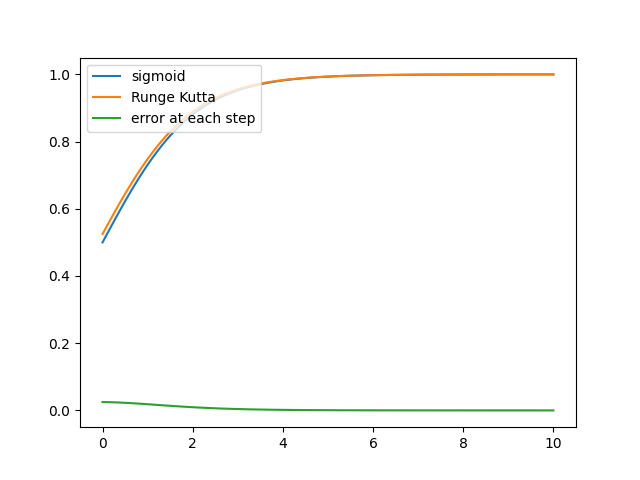
\includegraphics[width=.52\columnwidth]{Figures/rk4figure.png}} 
\subfloat[Euler's Method.]{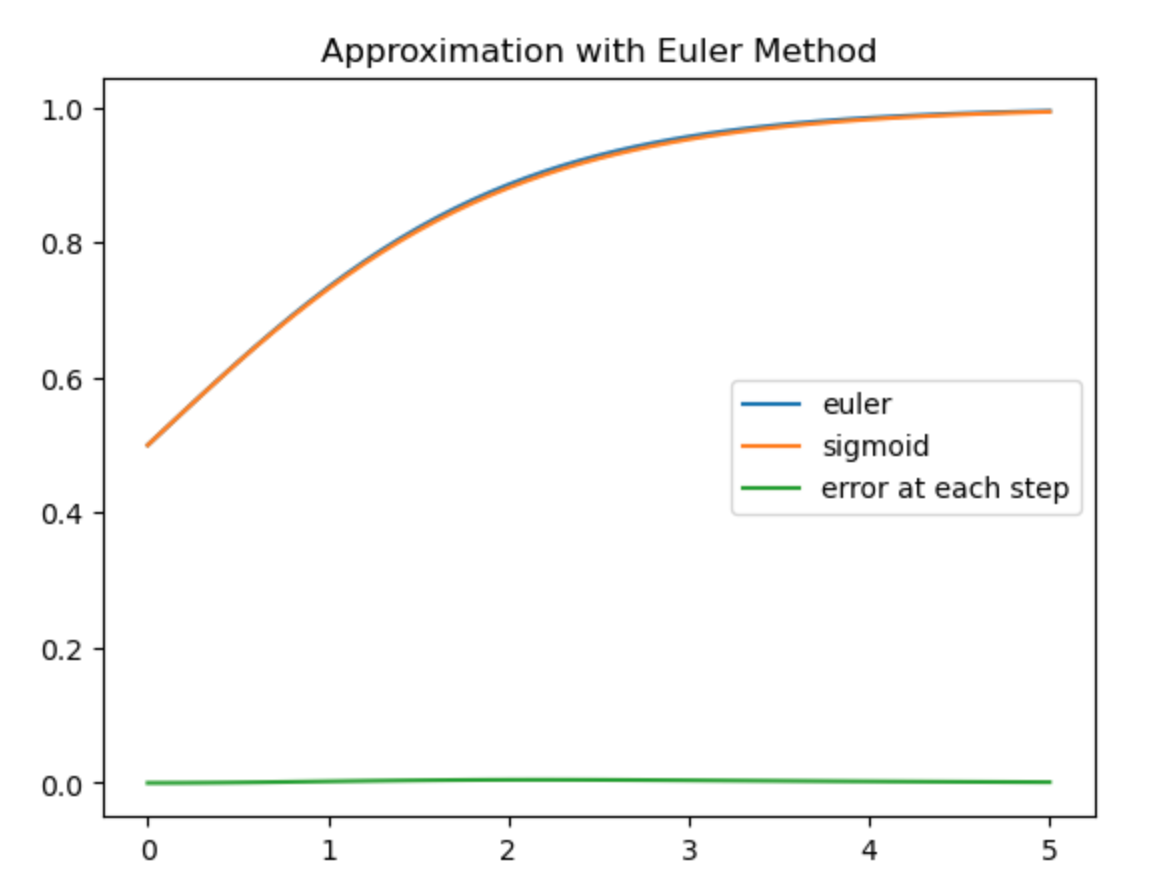
\includegraphics[width=.49\columnwidth]{Euler.png}} \\
\subfloat[Newton's Method.]{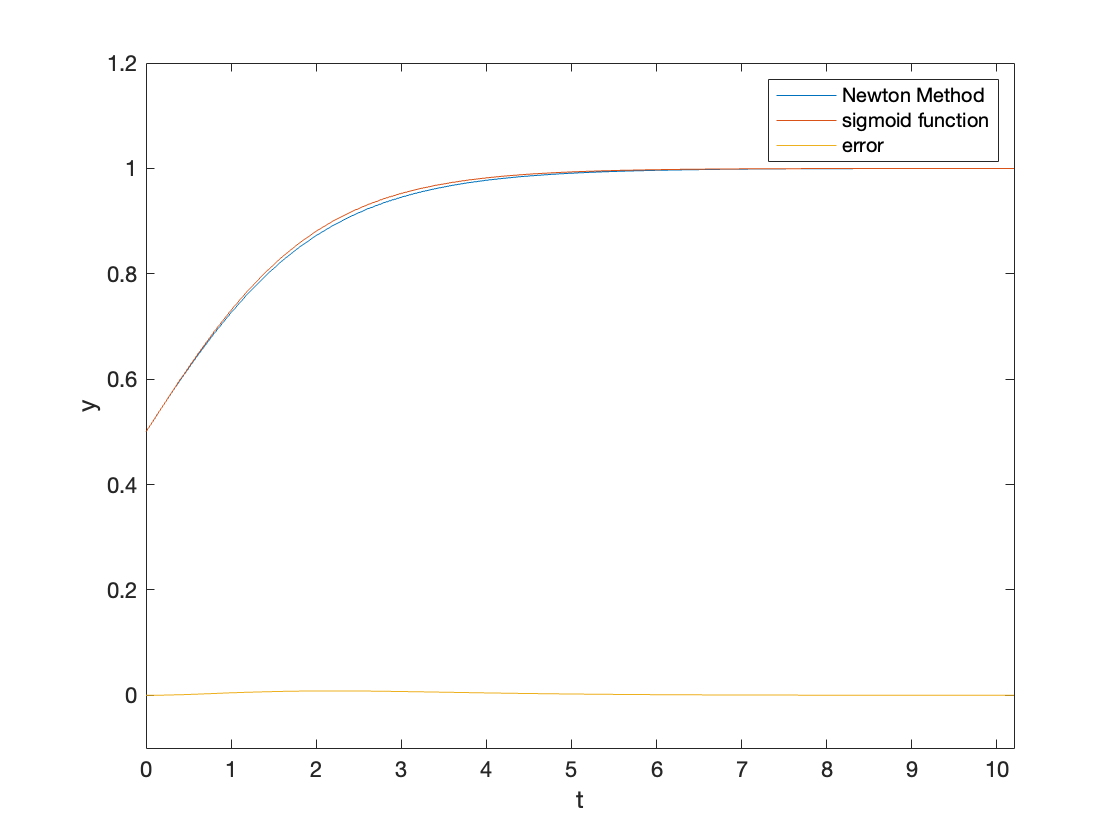
\includegraphics[width=.5\columnwidth]{newton.png}}\quad
\caption[error]{Iterated solution in $100$ iterations} 
\label{solution}
\end{figure}

\subsection{Runge-Kutta method}
Since the the most frequently used method of the Runge-Kutta family, the fourth-order Runge-Kutta method is generally superior to second order. Thus, we choose the fourth-order Runge-Kutta method here.\\
As an example, solution for $y_2$: \\
\begin{equation}
    f(y_n) = y_n - y_n^{2} \tag{3.3}
\end{equation}
when $n = 0$,
\begin{align}
     L_1 &= f(y_0) = \frac{1}{2} - \frac{1}{2}^{2} = 0.25 \notag \\
     L_2 &= f\left(y_0 + \frac{1}{2}hL_1\right) = f\left(\frac{1}{2} + \frac{1}{2}(0.1) \cdot \frac{1}{4}\right) = \frac{41}{80} - \frac{41}{80}^{2} \approx 0.2498 \notag \\
     L_3 &= f\left(y_0 + \frac{1}{2}hL_2 \right) = f\left(\frac{1}{2} + \frac{1}{2}\left(0.1\right)\cdot \frac{1599}{6400}\right) = f\left(\frac{65599}{128000}\right) \approx 0.2498 \notag \\
     L_4 &= f(y_0 + hL_3) = f\left(\frac{1}{2} + 0.1\cdot 0.2498\right) = f(0.52498) \approx 0.2494 \notag \\
     y_1 &= y_0 + \frac{h}{6}(L_1 + 2L_2 + 2L_3 + L_4) \approx 0.5250 \notag
\end{align}
When $n = 1$,
\begin{equation}
    L_1 = f(y_1) = 0.525 - 0.525^{2} \approx 0.2494 \notag
\end{equation}
\begin{equation}
    L_2 = f\left(y_1 +\frac{1}{2}hL_1\right) = f(0.5375) \approx 0.2486 \notag
\end{equation}
\begin{equation}
    L_3 = f\left(y_1 + \frac{1}{2}hL_2\right) = f(0.5374) \approx 0.2486\notag
\end{equation}
\begin{equation}
    L_4 = f(y_1 + hL_3) = f(0.5500) \approx 0.2374\notag
\end{equation}
\begin{equation}
    y_2 = 0.525 + \frac{1}{60}(0.2494 + 2\cdot 0.2486 + 2\cdot 0.2486 + 0.2374) \approx 0.5497 \notag
\end{equation}
Again, our implemented algorithm generated solution in Figure~\vref{solution} in $100$ times iteration.

\subsection{Newton method}
We start by using backward Euler method with $y_{n+1} = y_n + h(y_{n+1} - {y{n+1}}^2)$.\\
The goal is to build a function $F : y_{n+1} \rightarrow y_{n+1} - y_{n} - h(y_{n+1}-{y_{n+1}})^2$ such that $F(y_{n+1}) = 0$. i.e.,
\begin{center}
$F(y_{n+1}) = y_{n+1} - y_n -hf(y_n)$,\quad $f(y_n) = y_n - y_n^{2}$   
\end{center}
Then,
\begin{equation}
    F'(y_{n+1}) = 1 - h\frac{df(y_n)}{y_n} \notag
\end{equation}
So we use Newton Method, given $x_1 = y_n$,
\begin{equation}
    x_{n+1} = x_{n} - \frac{F(x_n)}{F'(x_n)} \tag{3.4}
\end{equation}
Note that since the Backward Euler's method's error is proportional to step-size's square, here we set the tolerance to be proportional to $h^2$. The resulted solution is shown in Figure~\vref{solution}.

\subsubsection{Variation on Step Size}
We now want to investigate the influence of step size $h$ on the convergence of each method. We do this by fixing iteration number at $100$ and vary the step size parameter $h$ from $0.05$ to $0.5$, then record the maximum error between the real solution (the sigmoid function) and the solution generated by each numerical method. Also, we compute the mean error on the interval at each $h$ within $100$ times of iteration as an additional reference.

\begin{table}[hbt]
\caption{Mean Error with Different Methods}
\centering
\begin{tabular}{ c c c c c c c }
\toprule
h & Euler & Newton & RK4 \\
\midrule
$0.05$ & $0.0023$ & $0.2752$ & $0.0125$ \\
$0.10$ & $0.0046$ & $0.1527$ & $0.0249$ \\
$0.15$ & $0.0071$ & $0.0692$ & $0.0370$ \\
$0.20$ & $0.0095$ & $0.0084$ & $0.0489$ \\
$0.25$ & $0.0120$ & $0.0424$ & $0.0603$ \\
$0.30$ & $0.0145$ & $0.0806$ & $0.0712$ \\
$0.35$ & $0.0171$ & $0.1114$ & $0.0816$ \\
$0.40$ & $0.0196$ & $0.1383$ & $0.0913$ \\
$0.45$ & $0.0225$ & $0.1606$ & $0.1003$ \\
$0.50$ & $0.0250$ & $0.1791$ & $0.1086$ \\
\bottomrule
\end{tabular}
\label{meanerror}
\end{table}
\begin{table}[hbt]
\caption{Maximum Error with Different Methods}
\centering
\begin{tabular}{ c c c c c c c }
\toprule
\multicolumn{2}{c|}{\multirow{2}{*}{1234}}
h & Euler & Newton & RK4 \\
\midrule
$0.05$ & $0.0006$ & $0.1029$ & $0.0048$ \\
$0.10$ & $0.0005$ & $0.0358$ & $0.0047$ \\
$0.15$ & $0.0005$ & $0.0129$ & $0.0046$ \\
$0.20$ & $0.0006$ & $0.0015$ & $0.0045$ \\
$0.25$ & $0.0006$ & $0.0056$ & $0.0044$ \\
$0.30$ & $0.0006$ & $0.0102$ & $0.0043$ \\
$0.35$ & $0.0006$ & $0.0136$ & $0.0041$ \\
$0.40$ & $0.0007$ & $0.0161$ & $0.0040$ \\
$0.45$ & $0.0007$ & $0.0180$ & $0.0039$ \\
$0.50$ & $0.0006$ & $0.0196$ & $0.0038$ \\
\bottomrule
\end{tabular}
\label{maxerror}
\end{table}
\vspace{0.6em} \noindent In order to investigate the tendency in $h$ more directly, we also separately plotted three graphs for error analysis for the three methods. Referring to Table~\vref{maxerror}, Table~\vref{meanerror}, and Figure~\vref{error}, we discover that for both Runge-Kutta Method and Euler's Method, mean error stays almost constant at different step size level, but maximum error increases enormously as step size grows. However, when operating Newton's Method, both mean error and maximum error reach minimum when $h \approx 0.2$ after normalization, while maximum error is influenced more seriously than mean error. 
\vspace{0.6em}\\From the above result, we could conclude that Runge-Kutta Method at order $4$ and Euler's Method operate more precisely for computing solutions to ODEs when step size is smaller, but one should be more careful when choosing the step size parameter for Newton's Method. 
\vspace{0.6em}\\ \textit{Remark} Choosing smaller step size cause higher computation complexity. It takes more steps for the algorithm to cover the interval we need, so one should choose a step size parameter considerably of the balance between computation time and preciseness.

\begin{figure}[tb]
\centering
\subfloat[Runge-Kutta Method at order $4$.]{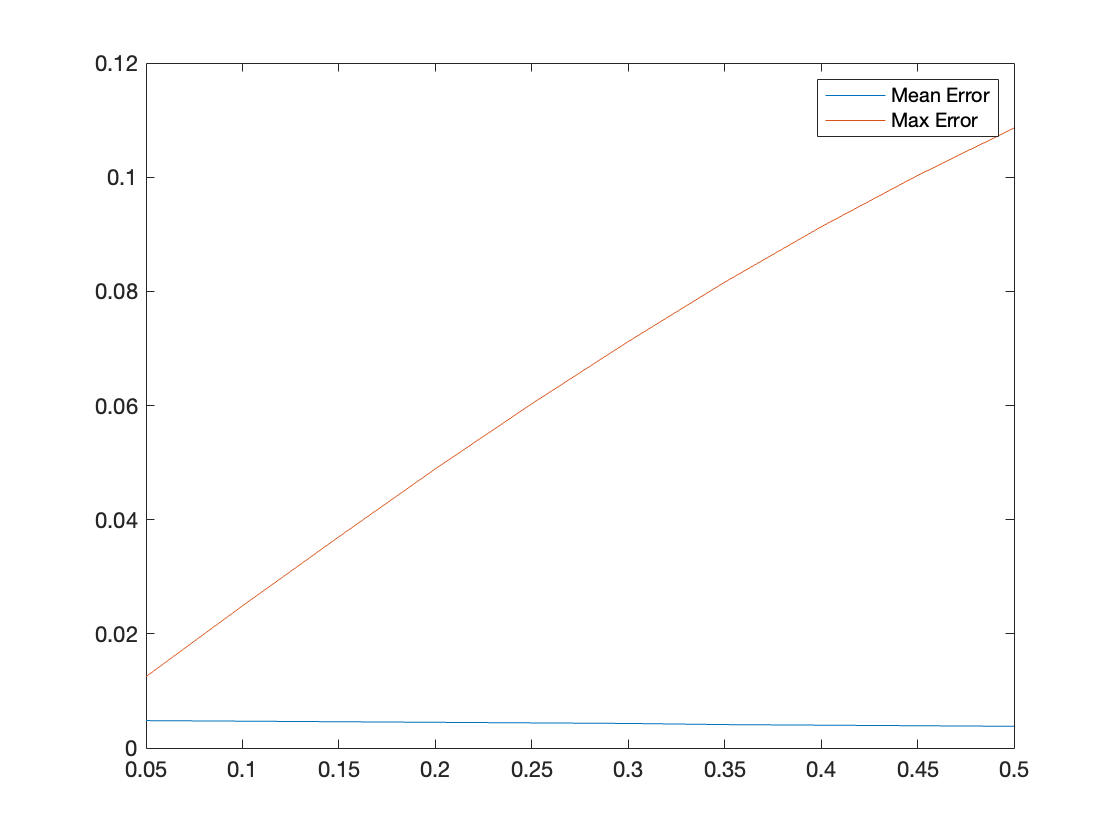
\includegraphics[width=.5\columnwidth]{rk4error.png}} 
\subfloat[Newton's Method.]{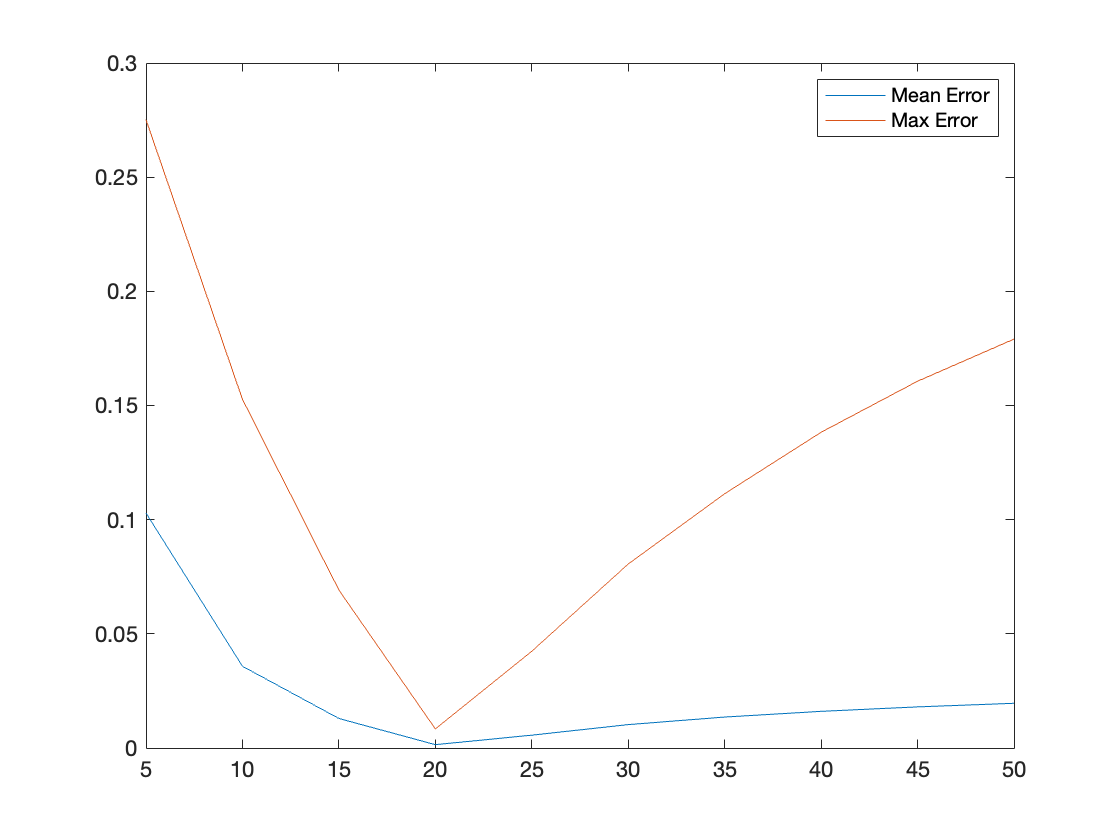
\includegraphics[width=.5\columnwidth]{newtonerror.png}\label{newtonerror}} \\
\subfloat[Euler's Method.]{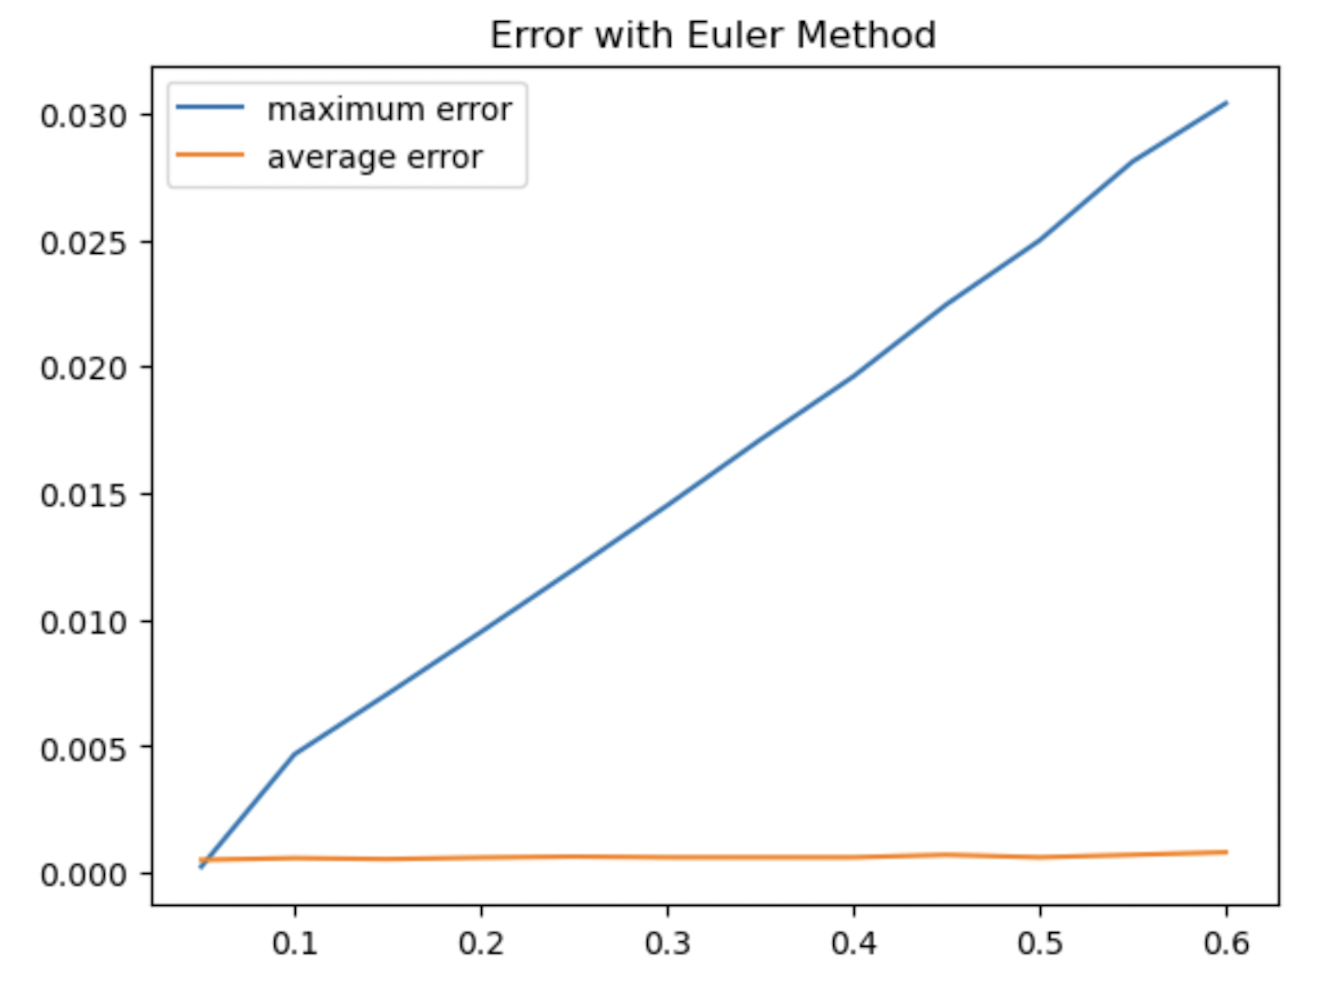
\includegraphics[width=.5\columnwidth] {eulererror.png}} \quad
\caption[error]{Error between exact solution and result from numerical schemes at different step size.} 
\label{error}
\end{figure}
\newpage




%----------------------------------------------------------------------------------------
%	BIBLIOGRAPHY
%----------------------------------------------------------------------------------------

\renewcommand{\refname}{\spacedlowsmallcaps{References}} % For modifying the bibliography heading


\bibliographystyle{unsrt}

\bibliography{refer.bib} % The file containing the bibliography

%----------------------------------------------------------------------------------------

\end{document}